\section{Background}
\label{rate-limiter:sec:background}


\subsection{Bandwidth Allocation and Rate Limiters}
\label{sec:bandwidth-allocation-in-clouds}
Bandwidth allocation is a must for cloud networks~\cite{shieh2011sharing,jeyakumar2013eyeq,rodrigues2011gatekeeper}. 
Software Rate limiters, e.g., Linux Traffic Control (TC), are the commonly used methods
to provide per-VM/container bandwidth allocation because of their flexibility and scalability.
In Linux traffic control, there are two kinds of rate limiting methods.
The first method is traffic shaping. In traffic shaping, packets are first pushed into a queue and delayed,
then packets are scheduled and sent to the network based on token and bucket-based mechanisms.
Shaping traffic ensures the traffic speed meets the desired rate.
A nice outcome of traffic shaping that it effectively makes bursty traffic
(TCP traffic is bursty because of offloading optimizations such TSO) more smooth.
Therefore, shaping traffic is good for switch buffers and avoid packet drops in the switches,
this is especially true because modern datacenter networks are built with shallow-buffered switches.
Another good property of traffic shaping is that it can effectively absorb bursty traffic and avoid
packet loss on the end-host.
The second rate limiting method is traffic policing. Traffic policing monitors the packet arrival rate,
it only pushes a packet into the queue when traffic rate is not above the desired rate,
otherwise the packet is dropped. Traffic policing is a less accurate and less effective
rate limiting method compared with traffic shaping~\cite{ovs-qos}.

\subsection{High throughput and Low Latency Datacenter Networks}
Datacenter networks need to support high throughput, low latency, and low loss rate to 
meet various kinds of application's SLAs. 
There have been many research work about reducing ``in-network'' 
latency and packet loss rate caused by network 
congestion~\cite{alizadeh2010data,he2016ac,mittal2015timely,zhu2015congestion,bai2015information,grosvenor2015queues}.
The work on reducing datacenter network latency can be roughly classified into two categories:
1) congestion control based such as DCTCP~\cite{alizadeh2010data} and DCQCN~\cite{zhu2015congestion}
and 2) priority-based such as PIAS~\cite{bai2015information} and QJUMP~\cite{grosvenor2015queues}. 
However, for bandwidth allocation functionality, prioritizing some flows is not realistic in a 
virtualized setting because the hypervisor has 
no way of knowing which VM traffic is more important.
Also, if high priority flows always come in, then low priority flows suffer from starvation.
Further, flows having the same priority still lead to queueing latency.
To date, little research effort has been done to explore latency, packet loss and burstiness 
issues of rate limiters on the end-host. 
We will show that queueing latency in the rate limiters on the end-host 
is not negligible, and it can increase end-to-end latency significantly. 
We will also demonstrate that end-host rate limiters have their own unique characteristics 
and we should rethink high throughput, low latency, and low loss rate solutions for end-host networking.


\iffalse
\wenfei{There is an argument here between Keqiang and me. Do we need to mention OVS ingress/egress
details here? I feel it is just an implementation issue.}

Today's datacenter servers host multiple VMs or containers to improve the utilization 
of computing resources. Different types of VMs and containers have different configurations 
(i.e., the number of cores, memory size, and network speed). High-end VMs and containers 
are typically sold at higher prices. To limit the network performance interference among 
different tenants on the same server, cloud providers need to provide 
bandwidth allocation~\cite{shieh2011sharing,jeyakumar2013eyeq}. 
The most commonly used approach is to provide per-VM or per-container bandwidth allocation. 
For example, on Google computing engine, different types of VMs are configured with different 
maximum bandwidths. To support a flexible and scalable bandwidth allocation among VMs and containers, 
software-based bandwidth management schemes such as Linux queueing disciplines are commonly employed. 
For example, Open vSwitch~\cite{openvswitch}, the most widely used open source virtual switch, supports two 
types of rate limiting schemes. The first one is ingress policing, which simply drops packets when 
a pre-configured maximum rate is exceeded. The approach is simple but less effective because 
of packet drops~\cite{ovs-qos}. 
\wenfei{``policing'' is the behavior of a rate limiter, not its position. 
At the ingress point, we can also configure a ``traffic shaping'' rate limiter, e.g., make the token bucket have a
large buffer: ``tc qdisc add dev br0 root tbf rate 8gbit latency 200ms burst 10000000000''. Here, I have a question,
ingress and egress points can both configured with traffic policing and shaping, why does OVS use policing at ingress
and shaping at egress? This is not explained at OVS web page. Any answer? Keqiang thinks this is not an important question
in this paper, we do not spend time on it.}
Packet loss has to be recovered from end-to-end, therefore it can lead to 
large flow completion times and the lost packets may need to wait for a coarse-grained 
TCP RTO to be retransmitted~\cite{alizadeh2010data,vasudevan2009safe}. 
The second and more effective approach is egress QoS 
(i.e., traffic shaping). Open vSwitch's egress QoS calls Linux queueing disciplines such as 
Hierarchical Token Bucket (HTB) to perform traffic shaping. Egress QoS absorbs bursty traffic 
and rate-limits each VM and container's bandwidth smoothly. Besides providing bandwidth allocation, 
it has been observed that traffic shaping can help reduce packet drops in shallow buffered switches 
which are widely used in modern datacenter networks~\cite{alizadeh2012less}. However, egress traffic shaping 
has a key drawback---it can increase network latency due to the queueing caused by 
software rate limiters (i.e., the queues in Linux queueing disciplines). 
That means we can not easily provide both bandwidth allocation and low latency.  


\subsection{Bandwidth Guarantee in Clouds}
\label{ssec:bandwidth-guarantee-in-clouds} \mylabel{ssec:bandwidth-guarantee-in-clouds}

\textbf{Token bucket based rate limiting.}
In current clouds, rate limiting is implemented based on token bucket algorithm. For example, current Linux system can configure a network device's  network scheduling algorithm (i.e., queuing discipline or qdisc) to be hierarchical token bucket (HTB) or token bucket filter (TBF). 
A token bucket based rate limiter maintains a queue, and is configured with two key parameters \textemdash\xspace \textit{rate} and \textit{burst}. ``Rate'' is the speed the limiter can send packets and ``burst'' is the queue length. All incoming packets are enqueued, and when they are dequeued and sent out, tokens are consumed; if no tokens are available, packets are queued; tokens are refreshed at the configured rate to enable packet dequeue; if queue length reaches or exceeds the configured length (i.e., burst), incoming packets are dropped.

\textbf{Traffic policing and shaping.~\cite{limitingandshaping}}
A token bucket with different queue length has different tolerance to bursty traffic. When bursty traffic incomes, smaller queue length causes excessive packets to be dropped, which is called \textit{traffic policing}. While larger queue length can buffer packets temporarily and sends packets out when tokens are refreshed, which is called \textit{traffic shaping}. 

\input{figs/policing_shaping_diagram.tex}
Figure~\ref{fig:policing-shaping-diagram} is a diagram showing the difference between traffic policing and shaping. The original traffic has a saw-tooth like shape, and its peak rate exceeds the configured rate. In traffic policing mode, excessive traffic is dropped, and in traffic shaping mode, it is buffered and the sending rate is smoothed.

\subsection{Measurement Results in Clouds}
\label{ssec:measurement-results} \mylabel{ssec:measurement-results}


\begin{figure*}[!htb]
\centering
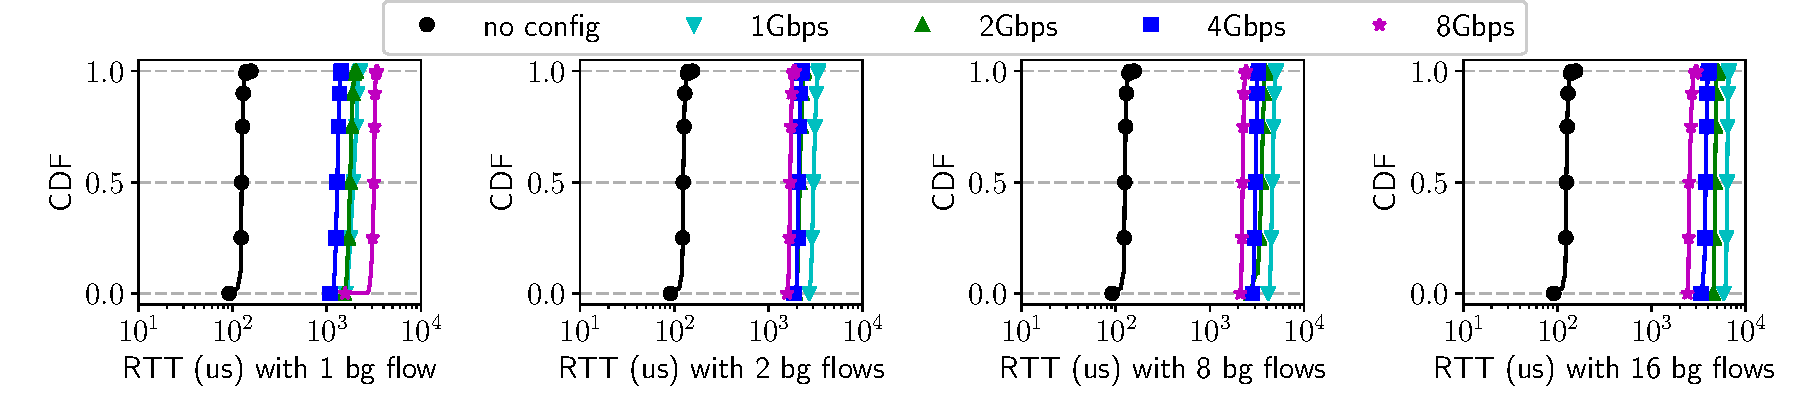
\includegraphics[width=\textwidth]{rate_limiter/raw_data/htb_benchmark/one_receiver.pdf}
\caption{HTB experiment: one receiver VM, varying rate limiting and number of background flows}
\label{fig:htb-1rec} 
\end{figure*}

\begin{figure*}[!htb]
\centering
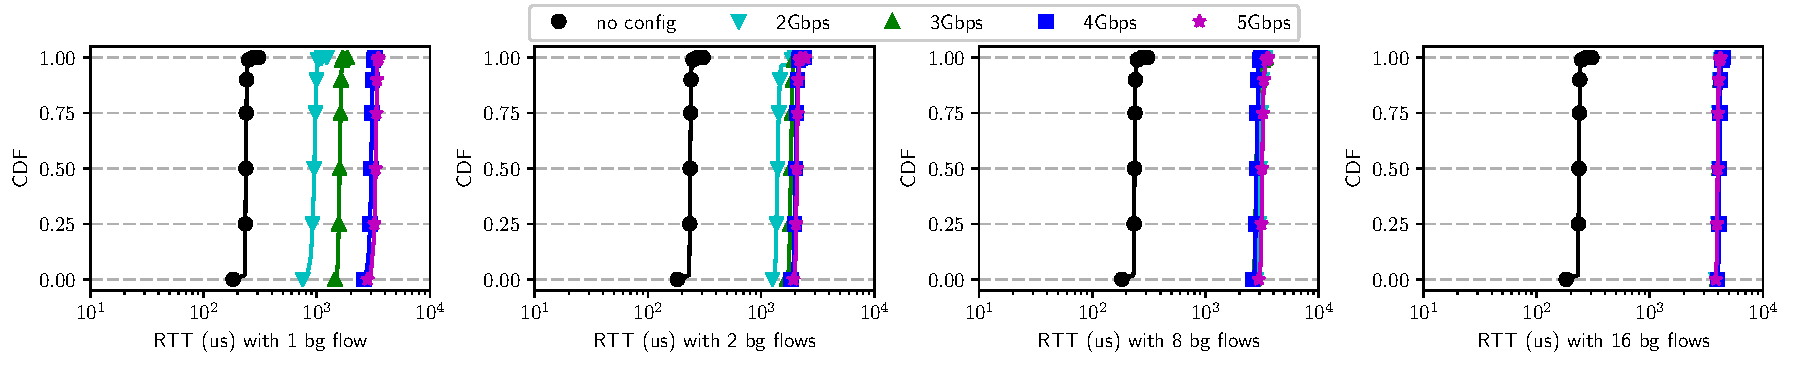
\includegraphics[width=\textwidth]{rate_limiter/raw_data/htb_benchmark/two_receivers.pdf}
\caption{HTB experiment: two receiver VMs, varying rate limiting and number of background flows}
\label{fig:htb-2rec} 
\end{figure*}



%\input{figs/latency_in_clouds.tex}
%\input{figs/buffer_vs_latency_of_rate.tex}


\wenfei{The figures here are placeholders, waiting for experiment results to fill in. If possible, we should also show drop.}


\fi
